\pagenumbering{arabic} %設定頁號阿拉伯數字
\setcounter{page}{1}  %設定頁數
\begin{center}
\fontsize{18}{16}\selectfont \textbf{介紹}\\
\end{center}
\fontsize{12pt}{2.5pt}\sectionef
\section{Process upgrade procedure 製程升級流程}
\fontsize{12}{2.5pt}\selectfont {The previous sections were about the procedure that would be necessary to use the Odoo software to track change during the main development of product. As such, most of what was described focused in the use of PLM and the standard procedure of creating and utilizing items like Products, BOMs, ECOs, MOs, WOs and Operations. This section will be different in the sense that now we have a production being carried out and the idea is to test Odoo in its capabilities of performing upgrades (Figure 59 and Figure 60). In other words, performance and feedback of information (and of course MES) becomes the main subject.}\\[1pt]

\fontsize{12}{2.5pt}\selectfont {前面的部分介紹了在產品主要開發過程中使用 Odoo 軟體追蹤變更所需的程序。 因此,所描述的大部分內容都集中在 PLM 的使用以及創建和利用產品、BOM、ECO、MO、WO 和營運等專案的標準程序。 本節將有所不同,因為現在我們正在進行生產,目的是測試 Odoo 執行升級的能力(圖 59 和圖 60)。 換句話說,訊息(當然還有MES)的表現和回饋成為主要課題。}\\[15pt]

\begin{figure}[hbt!]
\begin{center}
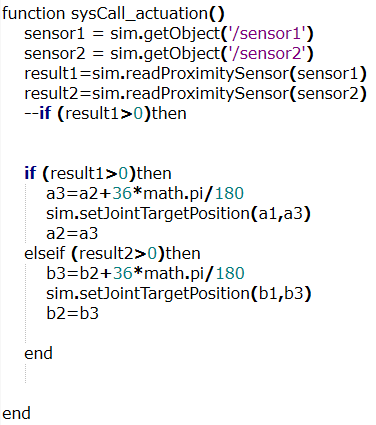
\includegraphics[width=15cm]{59}
\caption{\Large Sectioned diagram regarding Process upgrade procedure 有關流程升級程序的剖面圖}\label{fig.59}
\end{center}
\end{figure}

\begin{figure}[hbt!]
\begin{center}
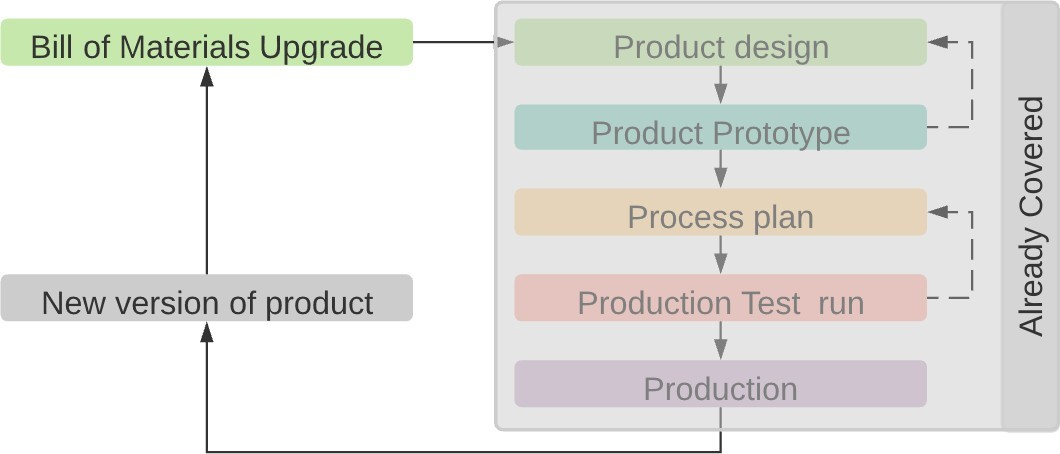
\includegraphics[width=15cm]{60}
\caption{\Large Sectioned diagram regarding Process development 有關流程開發的剖面圖}\label{fig.60}
\end{center}
\end{figure}

\fontsize{12}{2.5pt}\selectfont {Change is always enacted using the ECO functionality even in this case. To remind the reader the situation in which this change will be applied (Figure 61) is the product overview of the relevant product items. Every product item in that list (that is not a raw material) poses at least one BOM and two ECOs already applied to them in order to signify the initial state of every product item (Figure 62). The first ECO of every item affects the product and it holds the initial related files, the second is applied to the BOM of the product in order to hold files related to the initial state of the process as well as record the initial state of the BOM. Without these ECOs (Figure 62), when we ever applied an improvement, the initial state of the product files or BOMs would be lost.}\\[1pt]

\fontsize{12}{2.5pt}\selectfont {即使在這種情況下,也始終使用 ECO 功能來實施變更。 為了提醒讀者將套用此變更的情況(圖 61)是相關產品項目的產品概述。 此清單中的每個產品項目(不是原材料)至少包含一個 BOM 和兩個已應用於它們的 ECO,以表示每個產品項目的初始狀態(圖 62)。 每個專案的第一個 ECO 影響產品並保存初始相關文件,第二個 ECO 應用於產品的 BOM,以便保存與流程初始狀態相關的文件並記錄 BOM 的初始狀態。 如果沒有這些 ECO(圖 62),當我們應用改進時,產品檔案或 BOM 的初始狀態將會遺失。}\\[15pt]

\newpage
\begin{figure}[hbt!]
\begin{center}
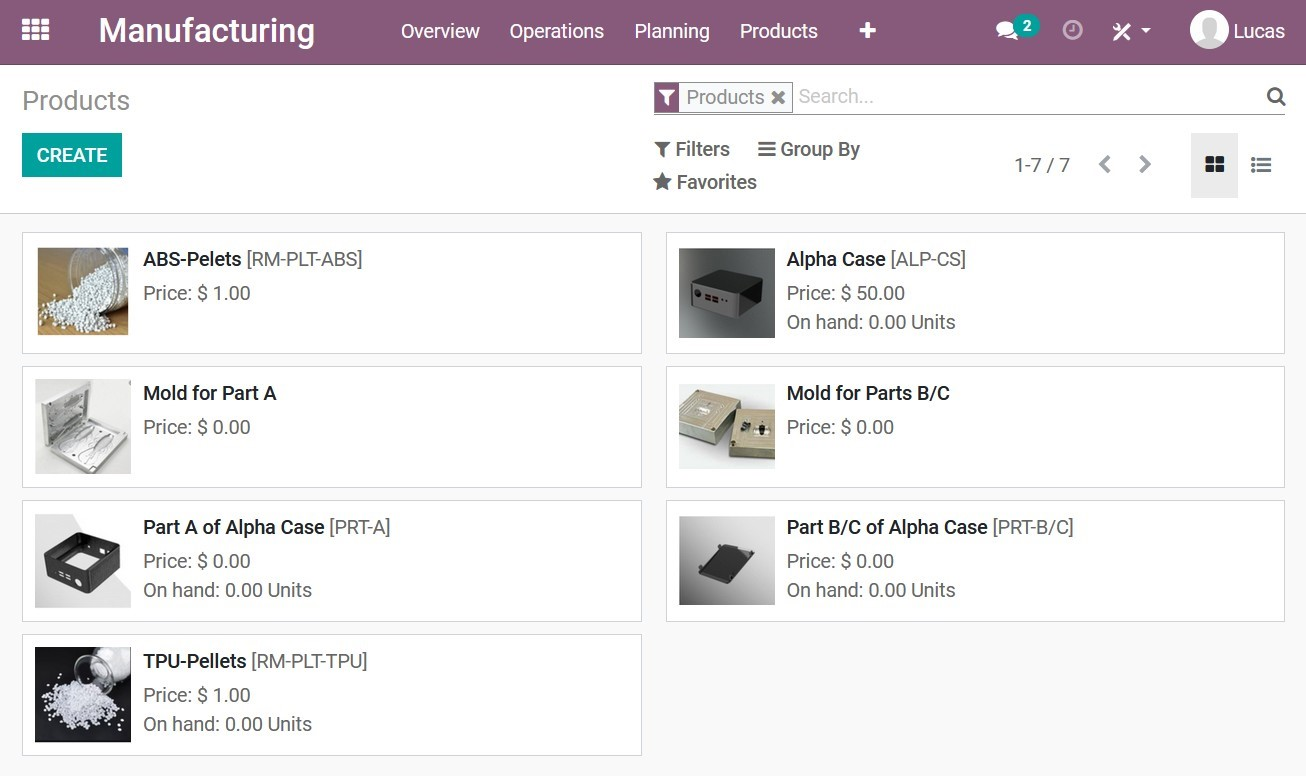
\includegraphics[width=15cm]{61}
\caption{\Large Relevant product items overview 相關產品項目概述}\label{fig.61}
\end{center}
\end{figure}
\newpage
\begin{figure}[hbt!]
\begin{center}
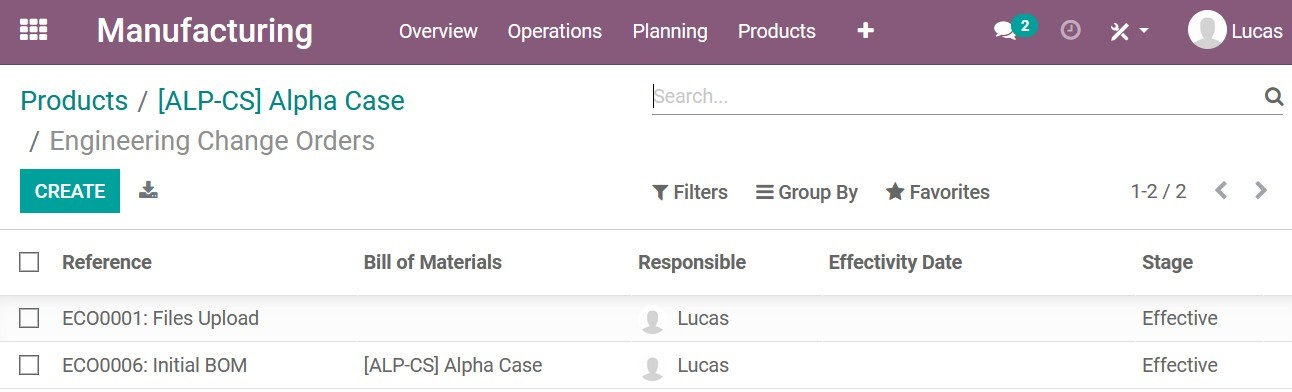
\includegraphics[width=15cm]{62}
\caption{\Large Example of ECOs of a product item 產品項目的 ECO 範例}\label{fig.62}
\end{center}
\end{figure}

\fontsize{12}{2.5pt}\selectfont {This time around the production duration and the estimated duration of the process is something that need to be taken in consideration so we can perceive how that applied change on the process affect production. To this end a MO of 50 units of Alpha Case will be created with each operation being estimated to take 30 seconds (15s for parts B/C because there is the need for 2 of them). Meaning that in an ideal situation the total length would be 50 minutes (25 of injection production being done in parallel and 25 for final assembly).In this simulated manufacturing run it was chosen that the injection operations would take slightly more time to complete to be representative of a suboptimal performance. This is been done to see how Odoo reacts and informs in real time the situation in hand.The first phase of the production in the injection process that is carried out in parallel for parts A and B/C on the injection stations 1 and 2. The following (Figure 64) shows how in the beginning of the process the overview of the productions stations indicate with green circles. These circulars signaling in known as Andon and although it is not always considered part of MES it is commonly an integrated feature in many MES systems. After the production process have been carried out with a little delay the circle turned gray and overall efficiency has been marked red on the station tabs (Figure 64).
}\\[1pt]

\fontsize{12}{2.5pt}\selectfont {這次需要考慮生產持續時間和流程的估計持續時間,以便我們能夠了解流程中應用的變更如何影響生產。 為此,將建立 50 個 Alpha Case 單元的 MO,每個操作預計需要 30 秒(B/C 部分需要 15 秒,因為需要其中 2 個)。 這意味著在理想情況下,總長度為 50 分鐘(25 分鐘的注射生產並行完成,25 分鐘用於最終組裝)。在此模擬製造運行中,選擇注射操作需要稍長的時間才能完成,以代表次優性能。 這樣做是為了了解 Odoo 如何反應並即時告知當前情況。注射過程的第一階段生產在註射站 1 和 2 上並行進行 A 和 B/C 部件。下圖(圖 64)顯示了在過程開始時的生產概覽車站以綠色圓圈表示。 這些循環訊號被稱為 Andon,儘管它並不總是被視為 MES 的一部分,但它通常是許多 MES 系統中的整合功能。 生產過程稍有延遲後,圓圈變為灰色,並且整體效率在工作站標籤上標記為紅色(圖 64)。}\\[15pt]

\begin{figure}[hbt!]
\begin{center}
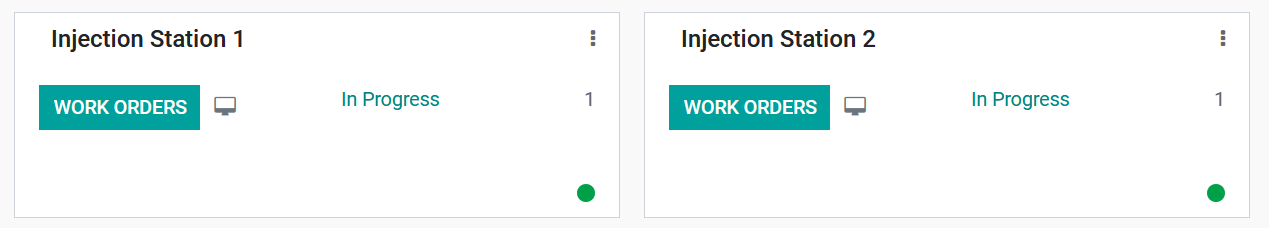
\includegraphics[width=15cm]{63}
\caption{\Large Workcenter overview 1 工作中心概述1}\label{fig.63}
\end{center}
\end{figure}

\begin{figure}[hbt!]
\begin{center}
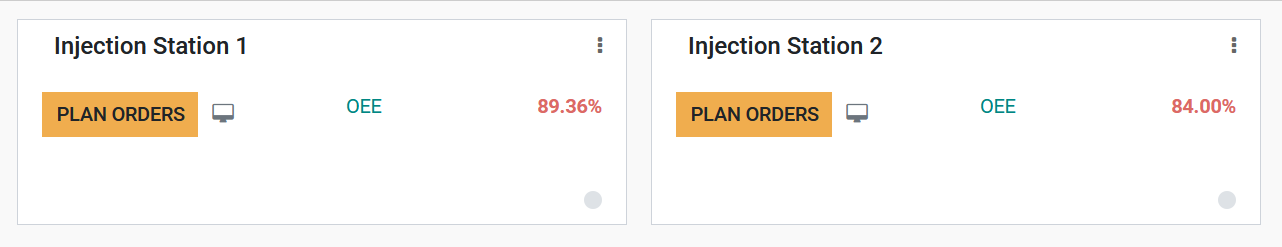
\includegraphics[width=15cm]{64}
\caption{\Large Workcenter overview 2 工作中心概述2}\label{fig.64}
\end{center}
\end{figure}

\fontsize{12}{2.5pt}\selectfont {The production was carried out twice before any improvement was applied. The first improvement to be carried out were on the production process on the operation and the raw materials used. More specifically, a new operation representative of an equipment upgrades on the injection machines and the replacement of the brand of plastic pellets use in the injection process (Figure 65).
}\\[1pt]

\fontsize{12}{2.5pt}\selectfont {在進行任何改進之前,生產進行了兩次。 首先要進行的改進是生產過程中的操作和所使用的原料。 更具體地說,新的操作代表了注射機的設備升級以及注射過程中使用的塑膠顆粒品牌的更換(圖 65)。}\\[15pt]

\begin{figure}[hbt!]
\begin{center}
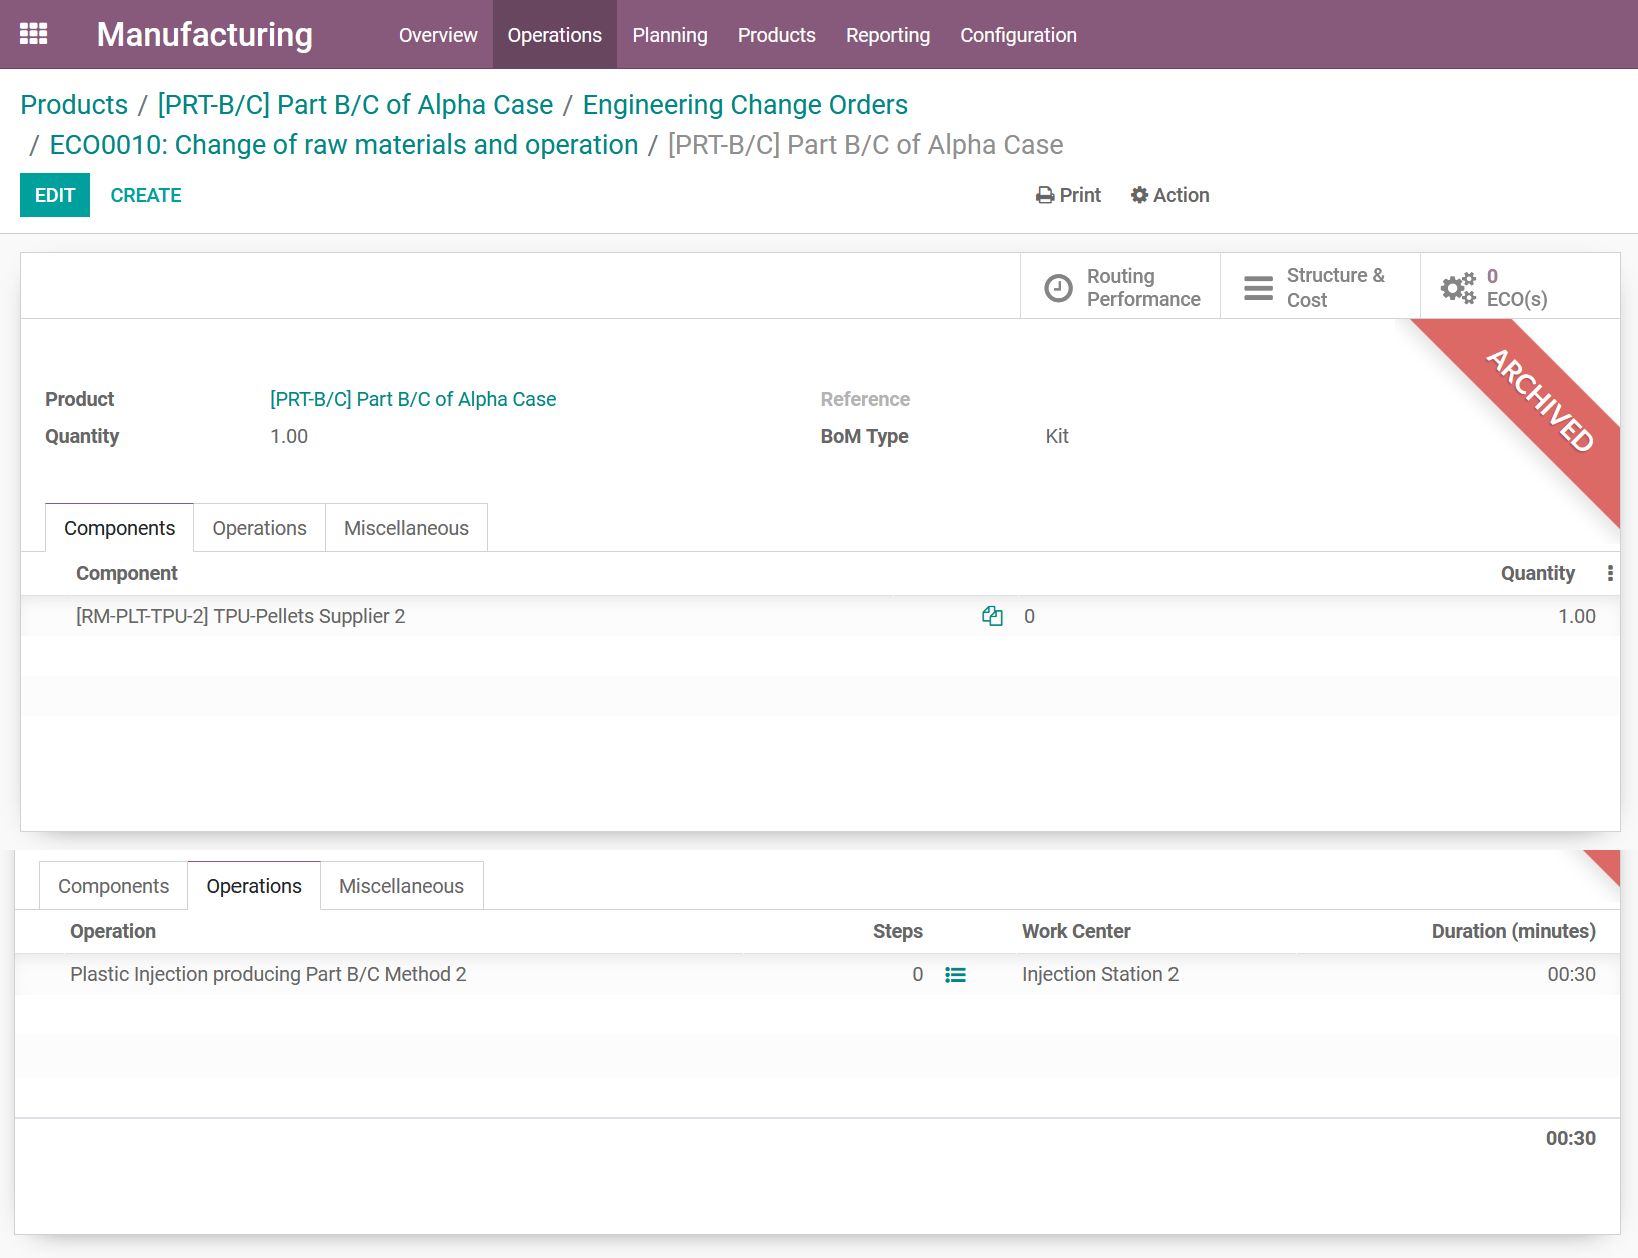
\includegraphics[width=15cm]{65}
\caption{\Large ECO applied to BOM ECO應用於BOM}\label{fig.65}
\end{center}
\end{figure}

\fontsize{12}{2.5pt}\selectfont {These upgrades were applied to the BOMs of parts A and B of the Alpha case and production recommenced. After two other MOs producing 50 products each simulating an improvement to the process the following types of data were automatically made available by Odoo (Table 3):}\\[1pt]

\fontsize{12}{2.5pt}\selectfont {這些升級已應用於 Alpha 機箱 A 和 B 部件的 BOM,並重新開始生產。 在另外兩個 MO 生產 50 個產品(每個產品模擬流程改善)後,Odoo 會自動提供以下類型的資料(表 3):}\\[15pt]

\begin{table}[htbp]
    \centering
    \label{tab:example}
    \begin{tabular}{|c|c|c|}
        \hline
        關於WO: & 關於 MO: &整體裝備\\
        \hline
            -持續時間偏差 &-缺貨順序 & -數量\\
       -每單位的持續時間 & -額外開銷& \\
       - 預計持續時間 & -生產數量& \\
        -數量 & -總數量& \\
 - 實際持續時間 &  & \\
    \hline
    \end{tabular}
\end{table}

\fontsize{12}{2.5pt}\selectfont {It should be commented that the data regarding MOs is unfortunately captured in a monthly basis as opposed to the other two categories that process data per order executed. This means that since this simulation is using a trial version of the software that lasts only 14 days the graphical representation of that data offers an unimpressive view of a single point or a single column. In the long run this is a great way to display performance over time but in the case of this simulation not so much (Figure 66).}\\[1pt]

\fontsize{12}{2.5pt}\selectfont {應該指出的是,不幸的是,與 MO 相關的數據是按月捕獲的,而不是按執行訂單處理數據的其他兩個類別。 這意味著,由於該模擬使用的軟體試用版僅持續 14 天,因此該資料的圖形表示提供了單點或單列的不起眼的視圖。 從長遠來看,這是顯示隨時間變化的性能的好方法,但在本次模擬的情況下效果並不好(圖 66)。}\\[15pt]

\begin{figure}[hbt!]
\begin{center}
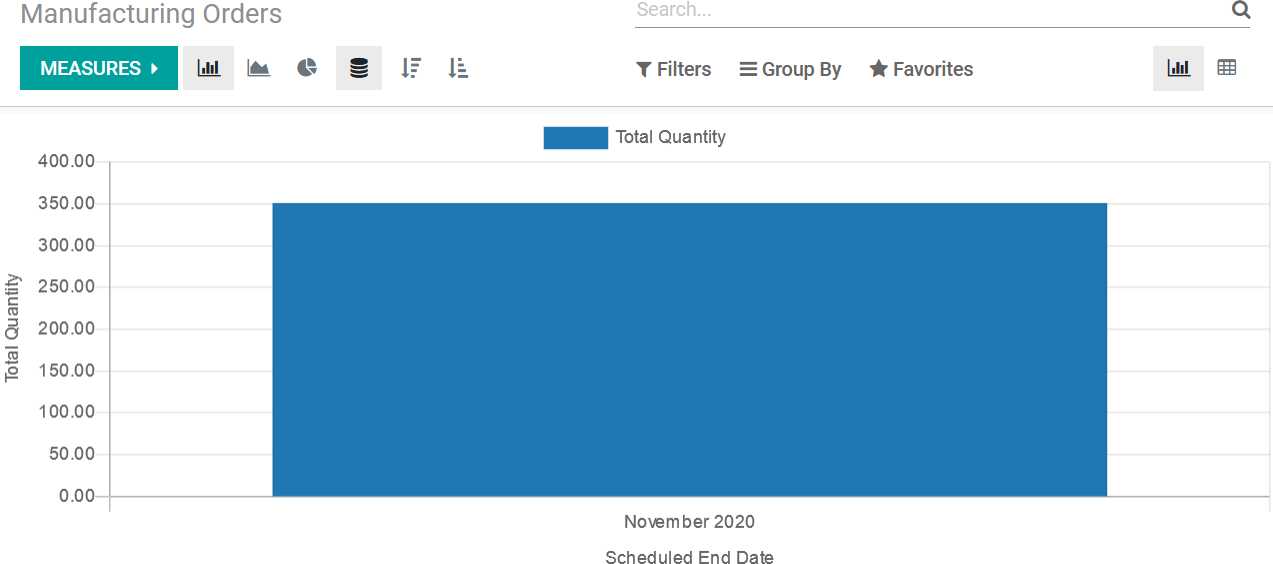
\includegraphics[width=15cm]{66}
\caption{\Large Total quantity regarding MO MO 總量}\label{fig.66}
\end{center}
\end{figure}

\fontsize{12}{2.5pt}\selectfont {All the data available can be seen in the form of bar charts, line charts or pie charts automatically generated after the time performance is registered (which happens at any moment an action is performed in a work order). Figure 67, Figure 68 and Figure 69 are examples of the results of the 5 production runs:}\\[1pt]

\fontsize{12}{2.5pt}\selectfont {所有可用資料都可以以長條圖、折線圖或圓餅圖的形式查看,這些資料是在註冊時間績效後自動產生的(在工單中執行操作的任何時刻都會發生)。 圖 67、圖 68 和圖 69 是 5 次生產運行的結果範例:}\\[15pt]

\begin{figure}[hbt!]
\begin{center}
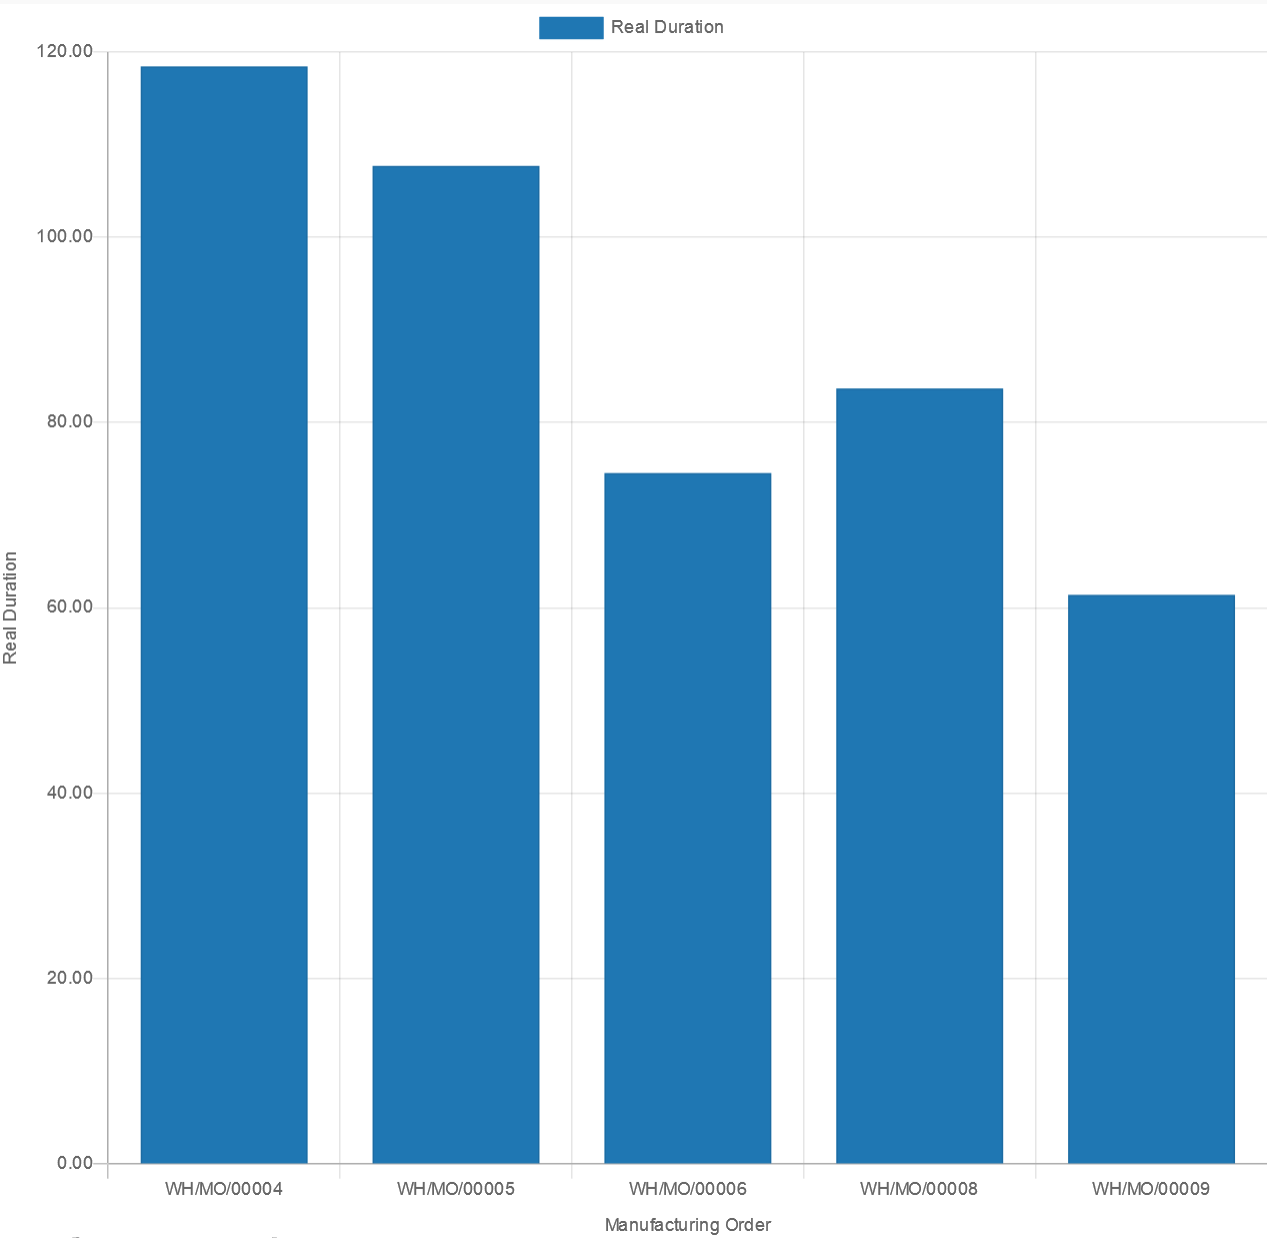
\includegraphics[width=15cm]{67}
\caption{\Large Real duration regarding work orders 有關工單的實際持續時間}\label{fig.67}
\end{center}
\end{figure}

\fontsize{12}{2.5pt}\selectfont {Something worth mentioning here is that whenever Odoo mentions quantity or duration it is referring to amount per workorder summed (the system does not care if the operations are being carried in parallel). So, on our simulation, making 50 units using 3 operations that should take 30 seconds each the estimated “duration” to be recorded ideally here is 75 minutes per MO.}\\[1pt]

\fontsize{12}{2.5pt}\selectfont {這裡值得一提的是,每當 Odoo 提到數量或持續時間時,它指的是每個工單的總金額(系統不關心操作是否並行進行)。 因此,在我們的模擬中,使用 3 次操作製造 50 個單元,每個操作應花費 30 秒,理想情況下,此處記錄的估計「持續時間」為每個 MO 75 分鐘。}\\[15pt]

\newpage
\begin{figure}[hbt!]
\begin{center}
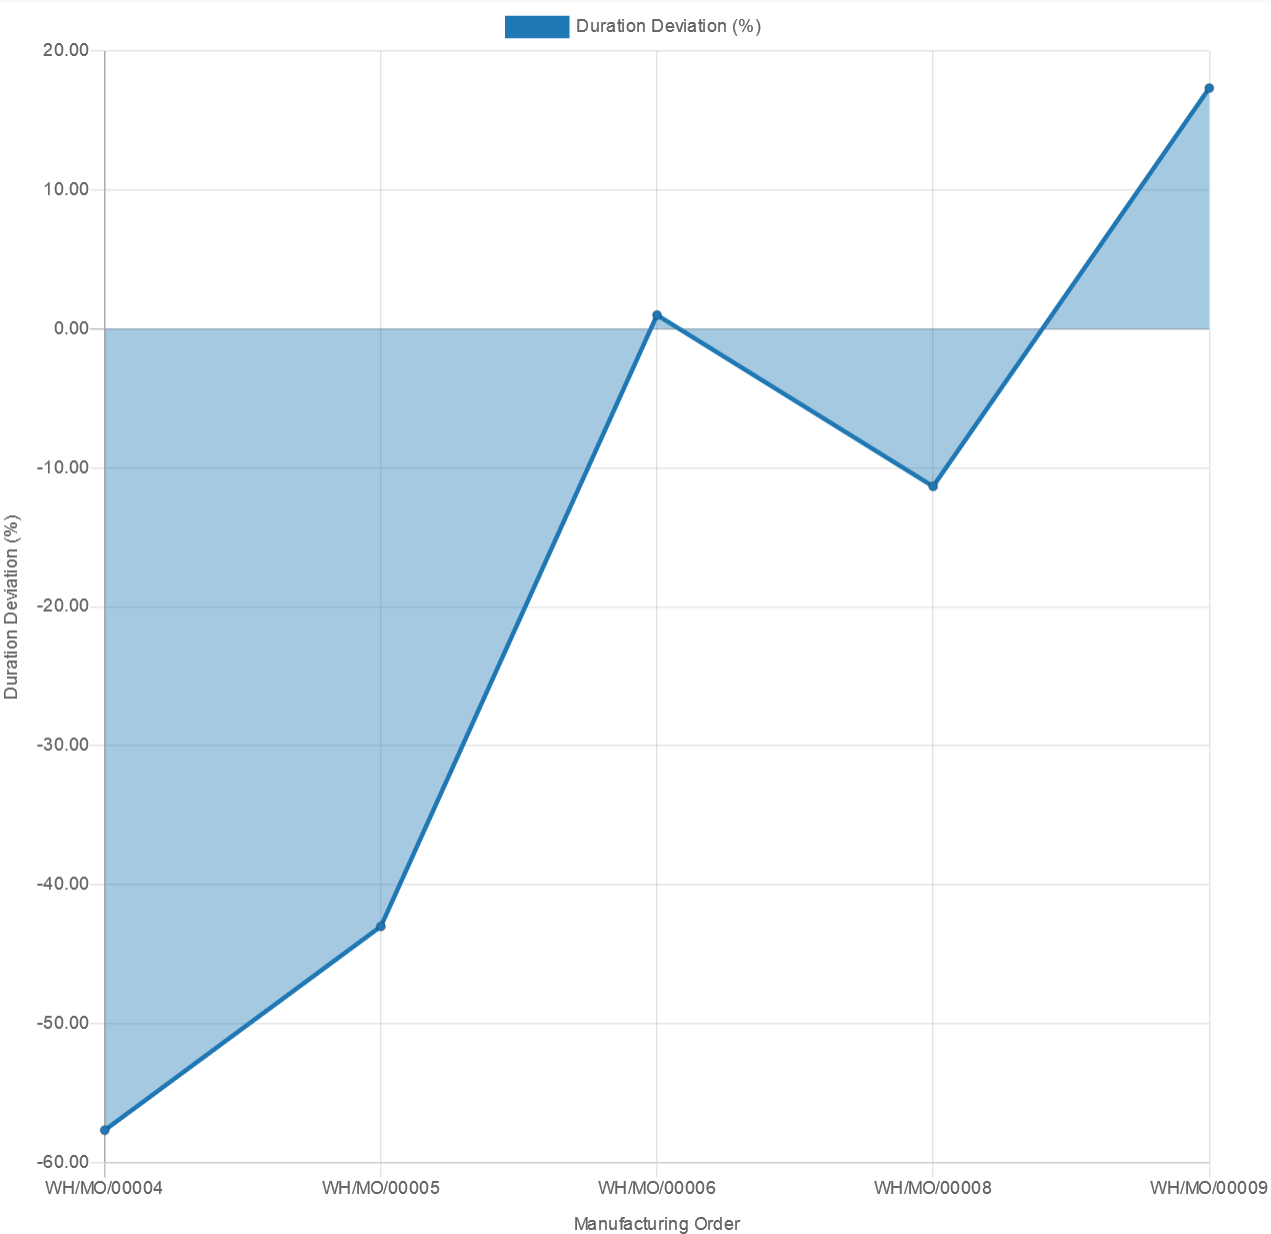
\includegraphics[width=15cm]{68}
\caption{\Large Duration variation regarding work orders 有關工單的持續時間變化}\label{fig.68}
\end{center}
\end{figure}

\newpage
\begin{figure}[hbt!]
\begin{center}
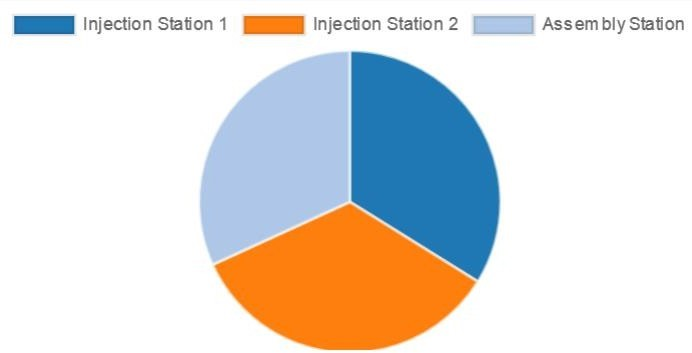
\includegraphics[width=15cm]{69}
\caption{\Large Overall equipment effectiveness 整體設備效率}\label{fig.69}
\end{center}
\end{figure}

\fontsize{12}{2.5pt}\selectfont {The astute reader will notice that all the data mentioned so far is derived from the time to completion of the operations been carried out, the related amount to the MO and the workcenter utilized. Even so it is impressive how much information can be drawn especially considering that it is all generated automatically.
}\\[1pt]

\fontsize{12}{2.5pt}\selectfont {精明的讀者會注意到,到目前為止提到的所有數據都是從完成作業的時間、與 MO 和所使用的工作中心相關的數量得出的。 即便如此,可以提取的資訊量仍然令人印象深刻,特別是考慮到這些資訊都是自動產生的。}\\[15pt]






